\documentclass[a4paper,11pt]{article}
\usepackage[utf8]{inputenc} % un package
\usepackage[francais]{babel} %active le mode francais
\usepackage[top=2cm , bottom=2cm , left=2cm , right=2cm]{geometry} %propriétés de notre page
\usepackage{amsmath} %liste de symboles et applications mathématiques
\usepackage{color} %Permet d'utiliser la couleur dans nos documents
\usepackage{listings} %Paquet de coloration syntaxique (langages)
\usepackage{hyperref} % Créer des liens et des signets 
\usepackage[babel=true]{csquotes} %permet les quotations (guillemets)
\usepackage{graphicx} %Importation d'image
\lstset{language=C}
% Informations du rapport
\title {Rapport \\ Travaux Pratiques Réseaux (Ethernet)}
\author {Quentin Tonneau - Adrien Lardenois}
\date{}
%Propriétés des liens
\hypersetup{
colorlinks=true, %colorise les liens  
urlcolor= blue, %couleur des hyperliens 
linkcolor= blue,%couleur des liens internes 
} 

\begin{document}
	\maketitle %insère l'en-tête du rapport
	\tableofcontents %insère la table des matières ATTENTION : Compiler deux fois en cas de changements
	\newpage % Nouvelle page
	
	
	\section{Introduction}
	Le but de ce projet est de fournir un logiciel capable de donner et d'évaluer le graphe de contrôle d'un programme écrit dans un pseudo langage ``simple''. Pour cela on met en place une interface très simple : on affiche un menu à choix multiple numéroté, le numéro choisi par l'utilisateur passe dans un ``switch'' qui execute les différentes actions correspondantes. On utilise un flag pour verifier qu'un fichier est bien en cours d'analyse pour éviter les erreurs.

	Pour la création du graphe en lui-même, nous avons  choisi une liste chainée. Chaque cellule contient :
	\begin{itemize}
		\item un sommet numéroté
		\item une étiquette (qui peut etre vide)
		\item la liste chainée des arêtes qui partent de ce sommet
		\item le lien vers la cellule suivante
	\end{itemize}
	Une cellule d'arête contient : 
	\begin{itemize}
		\item le numéro du sommet d'arrivée 
		\item une étiquette (normalement l'instruction permettant de passer par l'arête)
		\item la cellule arête suivante
	\end{itemize}
	
	L'utilisation d'une liste chainée de liste chainée permet de simplifier la manipulation de la mémoire tout en gardant une forte coherence des données, chaque liste d'arêtes étant attachée à son sommet d'origine. On dispose de fonctions pour ajouter des sommets et des arêtes, rechercher un sommet dans la liste, et enfin une fonction d'affichage du graphe.
	\subsection{Les fonctions d'ajout}
		L'ajout d'un sommet prend simplement le numéro et l'étiquette du sommet à créer ainsi que la liste à laquelle l'ajouter. On crée alors une nouvelle cellule et on l'ajoute en fin de liste, sauf pour une liste vide où elle devient la seule et unique cellule de la liste. En effet, l'utilisation par notre programme fait que jamais on ne créera deux sommets de même numéro et que les sommets sont créés en suivant une incrémentation régulière. Ainsi la liste proposera les sommets dans l'ordre de numérotation\footnote{qui pourra être différent de l'ordre d'éxecution, surtout dans les programmes contenant des conditionnelles.}

		L'ajout d'une arête passe par une fonction intermediaire. En apparence, on appelle \textbf{ajouter\_arete} avec pour arguments l'etiquette, le sommet de départ, le sommet d'arrivée et la liste de sommets. En fait, cette fonction n'est qu'un ``masque'' qui appelle \textbf{ajouter\_arete\_l} avec comme arguments : 
		\begin{itemize}
			\item l'etiquette
			\item la cellule du sommet de départ, donnée par \textit{recherche\_sommet(sommet\_d, liste)}
			\item le sommet d'arrivée
		\end{itemize}
		L'ajout se fait ensuite de façon standard, on crée une nouvelle cellule arête et on l'ajoute en tête de la liste d'arete.
	\subsection{Les fonctions de recherche et d'affichage}
		Ces deux fonctions reposent sur le même principe, on crée un clone de la liste que l'on parcours ensuite.

 Dans le cas de la recherche, on s'arrête dès que l'on trouve le sommet recherché ou que l'on est arrivé à la fin de la liste. Si on a effectivement trouvé on renvoie la cellule du sommet, sinon on ajoute le sommet à la liste et on rappelle la fonction à nouveau. Une utilisation normale n'appellera jamais de sommet inconnu mais nous avons fais ce choix afin d'eviter un blocage du programme en cas d'erreur.

	Dans le cas de l'affichage, le parcours se fait systematiquement jusqu'à la fin. Pour chaque sommet, on affiche sont numéro et son étiquette, puis on parcours sa liste d'arête de la même manière que la liste de sommet. A chaque arête, on affiche l'etiquette et le sommet d'arrivée, puis on passe à l'arête suivante. Quand la liste est finie, on passe au sommet suivant.

	\section{Ouverture et parsing}
		\textit{On considère dans la suite de ce rapport que le fichier d'entrée contient uniquement le programme, correctement syntaxifié.}
		
		Le code d'ouverture et de parsing du fichier se trouve dans les fichiers ``parser.c'' et ``parser.h''.
		\subsection{Ouverture du fichier}
		Le code permettant la lecture du fichier est simple, et commun à la plupart des applications réalisées en C. On note au passage que l'ouverture se fait en mode ``lecture'' uniquement.
		\begin{lstlisting}
FILE* fichier=NULL;
fichier=fopen(nomfichier,"r");
if(fichier==NULL)
{
	return 0; //on quitte le programme avec une erreur
}
		\end{lstlisting}
		\subsection{Parsing du fichier}
		L'algorithme repose sur une série de variable définies de la façon suivante :
		\begin{itemize}
		\item motlut : variable contenant le mot en cour de traitement (max. 50 caractères)
		\item instruction : concaténation des mots lus jusqu'à ``;''
		\item sommetactuel : numéro du dernier sommet créé
		\item nbsommet : nombre de sommet jusqu'à présent créés
		\end{itemize}
		Le parsing s'effectue à l'aide de la fonction fscanf, qui récupère un à un les mots contenus dans le fichier.
		\subsubsection{Cas général}
		Dans un fonctionnement général, c'est à dire un enchainement d'instructions sans conditionelle, l'algorithme concatène les mots lus jusqu'au symbole ';', puis crée une arête à l'aide de \textbf{ajouter\_sommet(nbsommet+1,graphe,"")} (sommet d'arrivée) puis \textbf{ajouter\_arete(instruction,sommetactuel,nbsommet,graphe)} dans laquelle nbsommet correspond au numéro du sommet tout juste créé.
		\subsubsection{Traitement des conditionnelles}
		Lorsque le programme rencontre le mot \textbf{Si}, il concatène l'ensemble des informations suivantes jusqu'au mot \textbf{Alors} dans une variable crée un sommet portant pour étiquette la chaîne précédement générée, le relie au graphique à l'aide d'une branche vierge.
		
		Il est important de décrire la manière dont les conditionelles sont traitées :\\
		L'algorithme possède un tableau d'entiers dans lequel on peut placer un numéro de sommet dont on nécéssite de conserver sa place. Le schéma suivant montre comment sont traitées les conditionelles :
		\begin{center}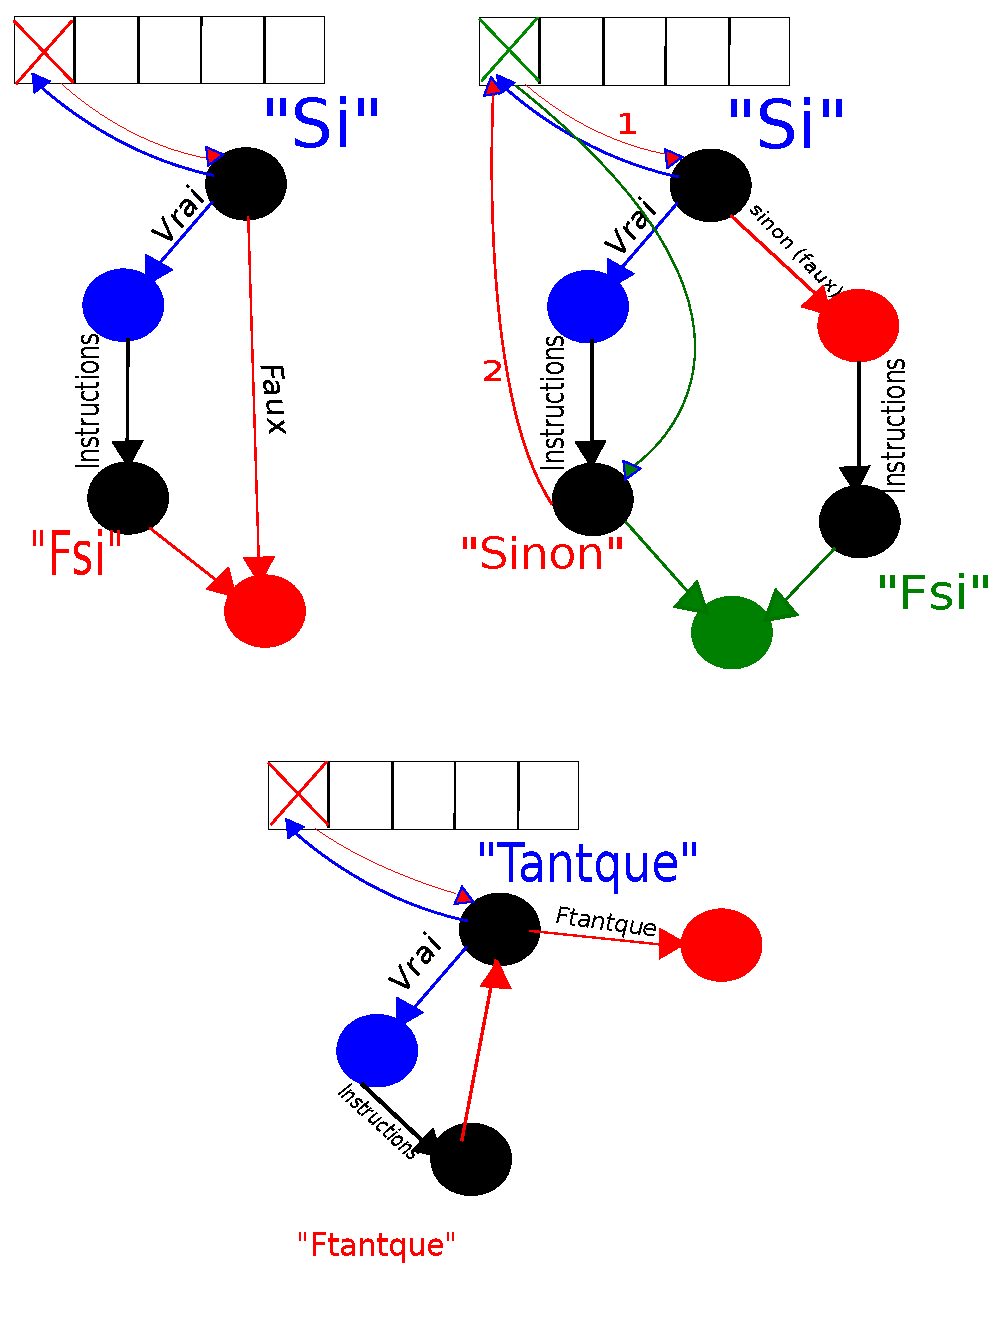
\includegraphics[width=15cm,height=15cm]{dessin.pdf}\end{center}
	On voit que le traitement du Fsi et du Ftantque (Rouge ou vert) est presque identique. Le programme récupère dans le tableau le sommet sauvegardé, créer un chemin vers (resp. depuis) ce dernier depuis (resp. vers) le dernier sommet créé, et continu le parsing. On remarque que quelque soit le type de conditionnelle, on utilise toujours une seule case de notre \textit{Tableau de sauvegarde}, et l'algorithme utilise toujours la dernière case de ce dernier. Ainsi, en cas d'imbrication de conditionnelles, le programme utilisera les cases suivantes, et les détruiras à la fin des traitements. Ainsi, en limitant à 50 la taille de notre tableau, nous limitons le nombre d'imbrication \textbf{maximum} à 50.
	\section{Analyse du graphe}
	\section{Pour aller plus loin}
	\section{Conclusion}

\end{document}
